Eight circles of diameter 1 are packed in the first quadrant of the coordinte plane as shown.  Let region $\mathcal{R}$ be the union of the eight circular regions.  Line $l,$ with slope 3, divides $\mathcal{R}$ into two regions of equal area.  Line $l$'s equation can be expressed in the form $ax=by+c,$ where $a, b,$ and $c$ are positive integers whose greatest common divisor is 1.  Find $a^2+b^2+c^2.$

\begin{center}
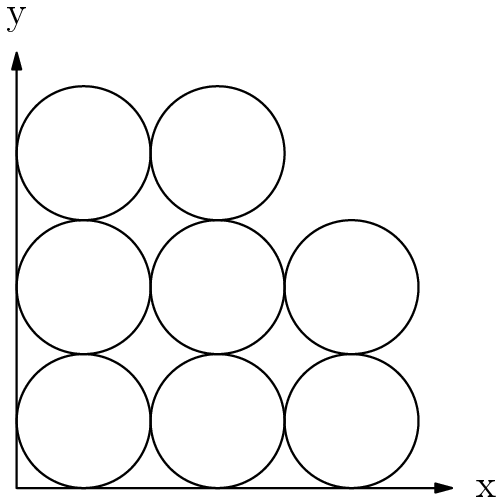
\includegraphics[width = 50.400000000000006mm]{img/fig0.png}
\end{center}